%!TEX root = main.tex
\begin{figure*}[!t]
\centering
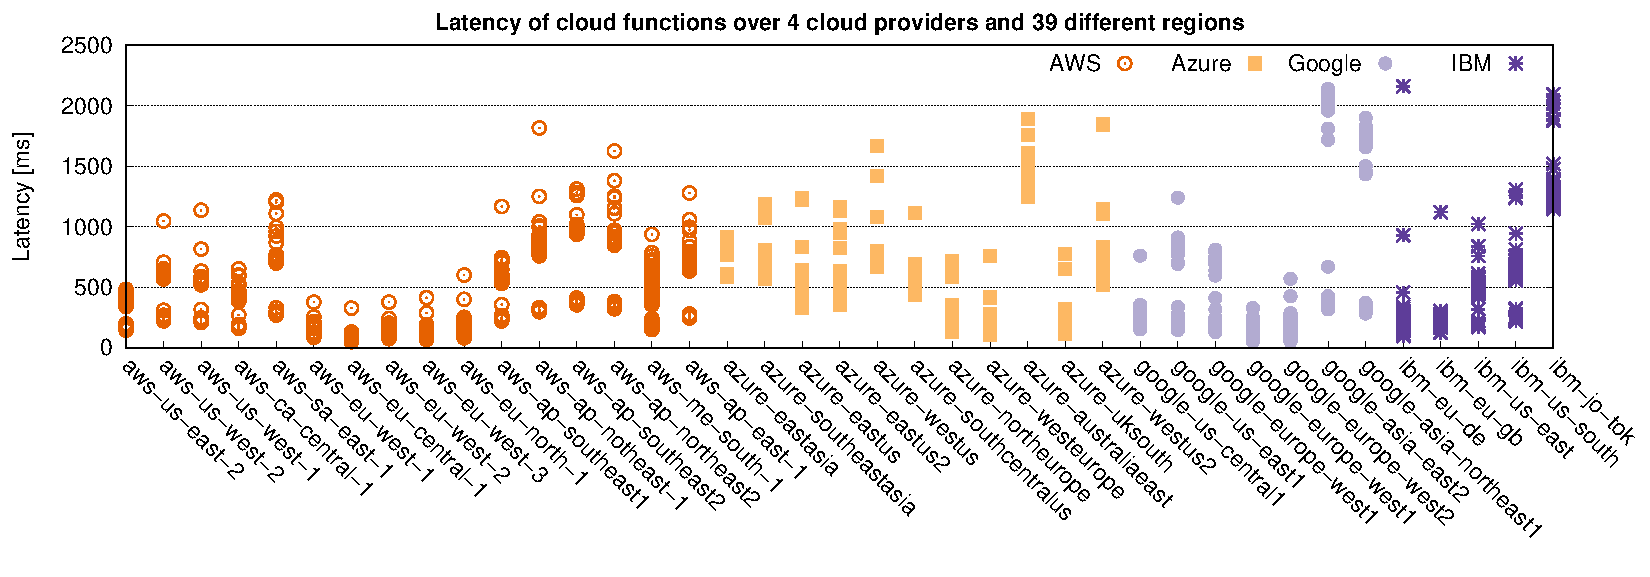
\includegraphics[width=1.0\textwidth]{bilder/latency/latency}
\caption{Latency test scatter plot. Since \texttt{azure-west-us} had issues with Node.js, we resort to \texttt{.NET} for that zone.}
\label{fig:latency_plot}
\end{figure*}
\section{The \sys Benchmark Suite}
\label{sec:tests}

The \sys benchmark suite consists of a collection of tests targeting different system aspects.
Each test is implemented in several programming languages in order to support the variety of the available runtime systems.
While there are some subtle differences across the code variants to adapt to the specificities of individual cloud providers, the code executed for each programming language is largely the same for all.
All functions are implemented using an \gls{HTTP} trigger, as supported by all the serverless providers.
Currently, \sys includes the followings benchmarks:

\textbf{\texttt{faas-fact}} and \textbf{\texttt{faas-matrix-mult}} are two CPU-bound benchmarks to respectively factorize an integer and multiply large integer matrices.

\textbf{\texttt{faas-netlatency}} is a network-bound test that immediately returns upon invocation, with a small \gls{JSON} payload (HTTP body of 79 bytes and HTTP complete response including headers of $\sim$500 bytes). This test is used to verify the roundtrip times for geographically distributed deployments

\textbf{\texttt{faas-diskio}} is an IO-bound benchmark to evaluate the performance of a disk. 
Perhaps surprisingly, each serverless cloud provides a temporary file-system that functions can use to read and write intermediate results. 
Other functions executed by the same instance share this file-system to access its content.

\textbf{\texttt{faas-custom}} is provided by \sys to allows developers to test custom functions. 
The suite provides templates for the currently supported cloud providers and the supported implementation languages. 
In the long term, we expect the number of custom functions to greatly outnumber those provided by the suite itself.



%\begin{itemize}
%\item \texttt{faas-fact} and \texttt{faas-matrix-mult}: two CPU-bound benchmarks, respectively to factorize an integer and to multiply large integer matrices;
%\item \texttt{faas-netlatency}: it immediately returns upon invocation, with a small \gls{JSON} (HTTP body ~ 79 bytes, HTTP complete response including headers around 500 bytes). This test is network-bound and useful to verify the roundtrip times for geographically distibuted deployments;
%\item \texttt{faas-diskio}: an IO-bound benchmark to evalute the performance of a disk. Perhaps surprisingly, each serverless cloud provides a temporary file system that functions can use to read/write intermediate results. 
%%The function can for example write a file with some intermediate results which it will later read again for further use. 
%Other function calls which run in the same instance share this file system and can access the same file. %Given that serverless tends to be or should be stateless, the feature of a temporary storage is not of great importance. 
%%Nevertheless, specific applications might benefit from such a feature and therefore it is included in this thesis. 
%I/O operations are typically expensive \vs{MAISSEN: any link to online catalogue of prices to show this?} \mais{In this case I didn't mean expensive money wise but regarding performance/execution (I/O operations are most times slower than CPU operations)} %and in a synchronous function that can lead to \gls{CPU} wait.
%\item \texttt{faas-custom}: our design allows developers to easily implement custom functions. 
%The suite provides templates for the currently supported cloud providers and the supported implementation languages. 
%In the long term, we expect the number of custom functions to greatly outnumber the ones provided by the suite itself.
%%Last but not least there is a customizable test. The objective of this test is that the user can easily implement his own function and then benchmark it. The skeleton is provided for each one of the four clouds in each of the four languages. A timer is included to measure the execution time which can later be further analysed.
%\end{itemize}



%This section will briefly explain all the implemented test functions, what they test and how they are implemented. 
%All the functions are implemented with a \gls{HTTP} trigger, since it is one that all clouds support and is the easiest to test across all platforms. 
%For the same programming language and the same test, the implementation will vary from cloud to cloud a little bit. 
%his is due to slightly different function calls and return statements each cloud defines on their own. However, these differences are not relevant regarding performance results.
%\subsection{Latency Test}
%\label{subsec:latency}
%The latency test  is fairly simple. 
%The function is called and then immediately returns a small \gls{JSON} body with \gls{HTTP} status code 200. The test function is intended to be as fast and simple as possible to measure latency for each cloud and runtime. 
%The following code listing \ref{code:latency} shows exemplary the implementation of the latency test on \gls{AWS} in Node.js.
%
%\begin{minipage}{\linewidth}
%\lstset{escapeinside={<@}{@>}}
%\begin{lstlisting}[frame=single,caption={Latency test implementation on AWS in Node.js},label=code:latency,linewidth=.82\textwidth,xleftmargin=.18\textwidth]
%  exports.handler <@\textcolor{javascriptbrown}{=}@> <@\textcolor{javascriptpurple}{function}@>(<@\textcolor{javascriptblue}{event}@>, <@\textcolor{javascriptblue}{context}@>, <@\textcolor{javascriptblue}{callback}@>) {
%      <@\textcolor{javascriptpurple}{const}@> <@\textcolor{javascriptblue}{res}@> <@\textcolor{javascriptbrown}{=}@> {
%          statusCode: <@\textcolor{javascriptroyalblue}{200}@>,
%          headers: {
%              <@\textcolor{javascriptred}{'Content-Type'}@>: <@\textcolor{javascriptred}{'application/json'}@>
%          },
%          body: JSON.stringify({
%              success: <@\textcolor{javascriptpurple}{true}@>,
%              payload: {
%                  <@\textcolor{javascriptred}{'test'}@>: <@\textcolor{javascriptred}{'latency test'}@>,
%              }
%          })
%      };
%    <@\textcolor{javascriptblue}{callback}@>(<@\textcolor{javascriptpurple}{null}@>, <@\textcolor{javascriptblue}{res}@>);
%  }
%\end{lstlisting}
%\end{minipage}
%
%\subsection{CPU Test (Factorization)}
%\label{sec:factors_test}
%This test describes the first of the two \gls{CPU} tests. 
%The \gls{CPU} is the component of a system which does effectively do the calculations of a program. 
%It is therefore the most important criterion of serverless computing and logically also the most expensive. This test is targeting mostly the \gls{CPU} by calculating all integer factors/divisors imperatively of an integer number. 
%Listing \ref{code:factors} shows pseudo code of such a number factorization.
%
%\begin{minipage}{\linewidth}
%\lstset{escapeinside={<@}{@>}}
%\begin{lstlisting}[frame=single,caption={Factorization test pseudo code},label=code:factors,linewidth=.75\textwidth,xleftmargin=.25\textwidth]
%  for(i = 1; i < SquareRoot(Number), i++) {
%      if(Number modulo i == 0) {
%          factors.add(i)
%          if(Number / i != i) {
%              factors.add(Number / i)
%          }
%      }
%  }
%\end{lstlisting}
%\end{minipage}
%
%The algorithm works as follows: one iterates from 1 to the square root of the number $N$ to be factorized. For each value $i$ it is tested if $N$ is dividable by $i$ without rest (modulo operator). If so, a factor of $N$ has been found and $i$ is added to the results. In addition, if $N$ divided by $i$ does not equal $i$ itself, the matching part $x$ of $i$ has also been found where $x \cdot i = N$. This is also the reason why only the numbers up to the square root of $N$ need to be considered. The algorithm has a complexity of $\mathcal{O}(n^{\frac{1}{2}})$.
%
%%\begin{remark}
%%The algorithm is not to be confused with prime factorization. In this case, all factors of a number are calculated but with prime factorization only prime numbers are calculated. 
%%The approach and results share some characteristics.
%%\end{remark}
%
%\subsection{CPU Test (Matrix Multiplication)}
%The matrix multiplication is the second \gls{CPU} test in this benchmark suite. 
%The user can input a number $n$ which defines the width and height of two matrices. The two matrices are both filled with random integer numbers between 0 and 100. 
%The product of those two matrices is calculated by multiplication. The algorithm is defined in listing \ref{code:matrix} in pseudo code.
%
%\begin{minipage}{\linewidth}
%\lstset{escapeinside={<@}{@>}}
%\begin{lstlisting}[frame=single,caption={Matrix multiplication test pseudo code},label=code:matrix,linewidth=0.8\textwidth,xleftmargin=.2\textwidth]
%  matrixA = randomMatrix[n][n]
%  matrixB = randomMatrix[n][n]
%  matrixMult = [n][n];
%  
%  for(i = 0; i < matrixA.height; i++) {
%      for(j = 0; j < matrixB.width; j++) {
%          sum = 0;
%          for(k = 0; k < matrixA.width; k++) {
%              sum += matrixA[i][k] * matrixB[k][j];
%          }
%          matrixMult[i][j] = sum;
%      }
%  }
%\end{lstlisting}
%\end{minipage}
%\newline
%
%First, two matrices of height and width $n$ are defined and filled with random integer numbers from 0 to 100. Also an empty matrix for the result is initialized. For each field of the resulting matrix one needs to calculate the dot product of row $i$ from matrix $A$ and column $j$ of matrix $B$. This is achieved by multiplying each field of row $i$ from matrix $A$ with each field of column $j$ from matrix $B$ and accumulating the sum over $k$. The sum is then stored as field $i,j$ in the resulting matrix. The algorithm has a complexity of $\mathcal{O}(n^{3})$.
%\subsection{I/O Test}
%The fourth test in this benchmark suite is a disk test. 
%Each serverless cloud provides a temporary file system which the functions can use. 
%The function can for example write a file with some intermediate results which it will later read again for further use. 
%Other function calls which run in the same instance share this file system and can also access the file. Given that serverless tends to be or should be stateless, the feature of a temporary storage is not of great importance. 
%Nevertheless, specific applications might benefit from such a feature and therefore it is included in this thesis. 
%I/O operations are often expensive and in a synchronous function that can lead to \gls{CPU} wait.
%%The implementation of the test is fairly simple. Listing \ref{code:filesystem} shows the pseudo code of the test.
%
%
%\begin{minipage}{\linewidth}
%\lstset{escapeinside={<@}{@>}}
%\begin{lstlisting}[frame=single,caption={I/O test pseudo code},label=code:filesystem,linewidth=0.75\textwidth,xleftmargin=.25\textwidth]
%  text = ""
%    
%  for(i = 0; i < s; i++) {
%      text += "A";
%  }
%  
%  startWrite = Time.Now()
%  for(i = 0; i < n; i++) {
%      writeFile(i+'.txt', text, 'utf-8');
%  }
%  endWrite = Time.Now()
%  
%  startRead = Time.Now()
%  for(i = 0; i < n; i++) {
%      file = readFile(i+'.txt', 'utf-8');
%  }
%  endRead = Time.Now()
%  
%  writeTime = endWrite - startWrite
%  readTime = endRead - startRead
%\end{lstlisting}
%\end{minipage}
%\newline

%The algorithm writes files and then reads them. 
%It takes two input parameters $n$ defining the number of files and $s$ the size of each file in bytes. 
%A string \texttt{text} is generated with length equal to $s$. 
%Since the encoding used is \texttt{utf-8} each normal character takes 8 bits or 1 byte of storage. 
%Then $n$ many files are written to the file system. 
%After that all the written files are read. 
%Both these operations are timed and the result will be the time it took to write respectively read the files.
%The complexity of the algorithm is $\mathcal{O}(n)$.

%\subsection{Custom Test}
%Last but not least there is a customizable test. The objective of this test is that the user can easily implement his own function and then benchmark it. The skeleton is provided for each one of the four clouds in each of the four languages. A timer is included to measure the execution time which can later be further analysed.